\begin{figure}[tbp]\centering
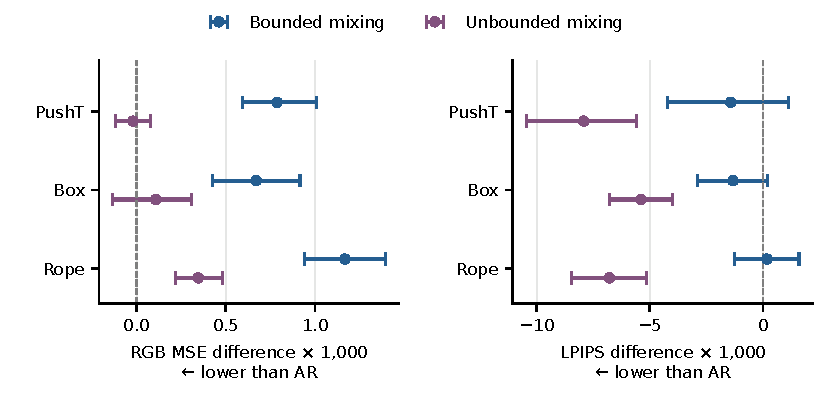
\includegraphics[width=\linewidth]{generated/iclr_review_v1/rgb_metric_tradeoffs.pdf}
\caption{Decoded endpoint conclusions depend on the metric. Points are named
mixing variant minus autoregression, with post-hoc paired trajectory--seed 95\%
bootstrap intervals, conditional on one fixed decoder per task. Negative favors
mixing. Unbounded mixing improves LPIPS relative to AR in all three tasks, but
its Rope RGB MSE is worse. Bounded mixing has worse RGB MSE in all tasks. Raw RGB
persistence has lower LPIPS than every decoded predictor and is retained in
Table~\ref{tab:rgb-endpoint-comparison}; these panels are not an all-baseline
superiority claim.}
\label{fig:rgb-metric-tradeoffs}\end{figure}
